\documentclass[lettersize,journal]{IEEEtran}
\usepackage{amsmath,amsfonts}
\usepackage{algorithmic}
\usepackage{algorithm}
\usepackage{array}
\usepackage[caption=false,font=normalsize,labelfont=sf,textfont=sf]{subfig}
\usepackage{textcomp}
\usepackage{stfloats}
\usepackage{url}
\usepackage{verbatim}
\usepackage{graphicx}
\usepackage{cite}
\hyphenation{op-tical net-works semi-conduc-tor IEEE-Xplore}
% updated with editorial comments 8/9/2021

\begin{document}

\title{Procesamiento Digital de Señales para la Detección del Evento de Ondas Gravitacionales GW170814}

\author{Karen Ingala,~\IEEEmembership{Procesamiento Digital Multimedia,~    EIE 401,}
        % <-this % stops a space
\thanks{This paper was produced by the IEEE Publication Technology Group. They are in Piscataway, NJ.}% <-this % stops a space
\thanks{Manuscript received April 19, 2021; revised August 16, 2021.}}

% The paper headers
\markboth{EIE 401: Procesamiento Digital de Multimedia, Mayo 2026}{Proyecto 1: Análisis de Ondas Gravitacionales}


% Remember, if you use this you must call \IEEEpubidadjcol in the second
% column for its text to clear the IEEEpubid mark.

\maketitle

\begin{abstract}
Este artículo describe el procesamiento digital del evento de ondas gravitacionales GW170814 utilizando datos de la colaboración LIGO-Virgo. El estudio aborda la optimización de la relación señal-ruido (SNR) mediante una metodología que incluye la mitigación de fugas espectrales con una ventana de Hann, superando las deficiencias de la ventana rectangular tradicional. Se implementó un proceso de blanqueo (whitening) y filtrado Butterworth (30-400 Hz) para aislar la señal astrofísica, seguido de un resampleo a 8 kHz para incrementar la resolución temporal. Los resultados confirman la detección de la morfología tipo 'chirp' en el intervalo $t=9.8s$ a $t=10.0s$, validada mediante análisis de espectrogramas y verificación auditiva. El trabajo demuestra la eficacia del procesamiento multirresolución en la identificación de transitorios de alta energía en entornos ruidosos.
\end{abstract}

\begin{IEEEkeywords}
Ondas gravitacionales, GW170814, Procesamiento digital de señales, Ventana de Hann, Espectrograma, Resampleo, LIGO.
\end{IEEEkeywords}

\section{Introduction}
\IEEEPARstart{E}El estudio de las ondas gravitacionales es un reto importante porque estas señales son muy débiles y llegan a la Tierra mezcladas con mucho ruido de los instrumentos. El evento GW170814 es especial porque fue uno de los primeros detectados por tres observatorios distintos al mismo tiempo, lo que permitió confirmar con mayor claridad el choque de dos agujeros negros\cite{gw170814}.

En este trabajo, el objetivo es procesar los datos crudos de ese evento usando Python para 'limpiar' la señal. El problema principal es que el ruido del detector es muy fuerte y oculta la forma de la onda. Para solucionar esto, aplicamos un flujo de trabajo que incluye el análisis de Fourier para entender las frecuencias de ruido y técnicas de filtrado para aislar el famoso chirp. Al final, buscamos que la señal se pueda ver en gráficas y también escuchar, validando así que el procesamiento fue exitoso.

\section{Marco Teórico}
En esta sección se describen los pilares técnicos utilizados para el procesamiento de la señal GW170814:

\begin{itemize}
    \item \textbf{Análisis de Fourier y Windowing:} La Transformada de Fourier permite descomponer la señal en sus componentes de frecuencia. Para evitar el "efecto peine" o fugas espectrales que ocurren al cortar los datos brutos, se aplica una ventana de \textit{Hann}. Esta función suaviza los extremos de la serie de tiempo, asegurando que la potencia del ruido sea representada de forma correcta.

    \item \textbf{Análisis de Fourier y Windowing:} La Transformada de Fourier permite descomponer la señal en sus componentes de frecuencia. Para evitar las fugas espectrales, se aplica una ventana de \textit{Hann}, definida matemáticamente como:

\begin{equation}
w(n) = 0.5 \left( 1 - \cos \left( \frac{2\pi n}{M-1} \right) \right)
\end{equation}

Donde $n$ es la muestra actual y $M$ es el número total de puntos. Esta función asegura que los extremos de la señal lleguen a cero suavemente, eliminando el "efecto peine"\cite{oppenheim}.
    
    \item \textbf{Blanqueo (Whitening):} Dado que el ruido de los detectores LIGO no es uniforme (ruido coloreado), el blanqueo normaliza los datos para que el ruido tenga una potencia constante en todas las frecuencias. Esto facilita que la señal del evento astronómico "sobresalga" visualmente sobre el fondo ruidoso.
    
    \item \textbf{Filtrado Digital:} Se utiliza un filtro pasabanda (Butterworth) para eliminar frecuencias fuera del rango de interés ($30$ a $400$ Hz). Esto descarta ruidos de baja frecuencia (sismos o vibraciones) y de alta frecuencia que no pertenecen a la colisión de agujeros negros.
    
    \item \textbf{Resampleo:} El incremento de la frecuencia de muestreo a $8000$ Hz permite una reconstrucción más suave de la onda. Esto mejora la resolución para el análisis del espectrograma y permite generar un audio de alta fidelidad para la validación auditiva del \textit{chirp}.
\end{itemize}

\section{Metodología}
El procesamiento de los datos se realizó en el entorno de Python siguiendo cuatro etapas principales:
\begin{enumerate}
    \item \textbf{Preparación y Carga de Datos:} Se importó la serie de tiempo del detector de Hanford, obtenida del portal abierto de LIGO (GWOSC) \cite{gwosc}, correspondiente al evento GW170814. Se definieron los parámetros base, incluyendo la frecuencia de muestreo original de $4000$ Hz y el tiempo central del evento detectado ($t \approx 9.77$ s).
    
    \item \textbf{Tratamiento Espectral:} Se calculó la Densidad Espectral de Potencia (PSD) comparando el uso de una ventana rectangular frente a una de \textit{Hann}. Posteriormente, se aplicó un blanqueo (\textit{whitening}) para normalizar el ruido del instrumento y un filtro Butterworth pasabanda de orden 4 entre $30$ y $400$ Hz para aislar la señal astronómica.
    
    \begin{figure}[htbp]
    \centering
    \includegraphics[width=0.45\textwidth]{psd.png}
    \caption{Densidad Espectral de Potencia (PSD) comparando el efecto de la ventana Rectangular vs. Hann.}
    \label{fig:psd}
\end{figure}
    
    \item \textbf{Resampleo:} Con el fin de mejorar la definición de la onda y la calidad del audio final, se incrementó la frecuencia de muestreo a $8000$ Hz mediante interpolación polifásica. Este paso permitió obtener una reconstrucción más suave de los picos de amplitud de la señal procesada.
    \begin{figure}[htbp]
    \centering
    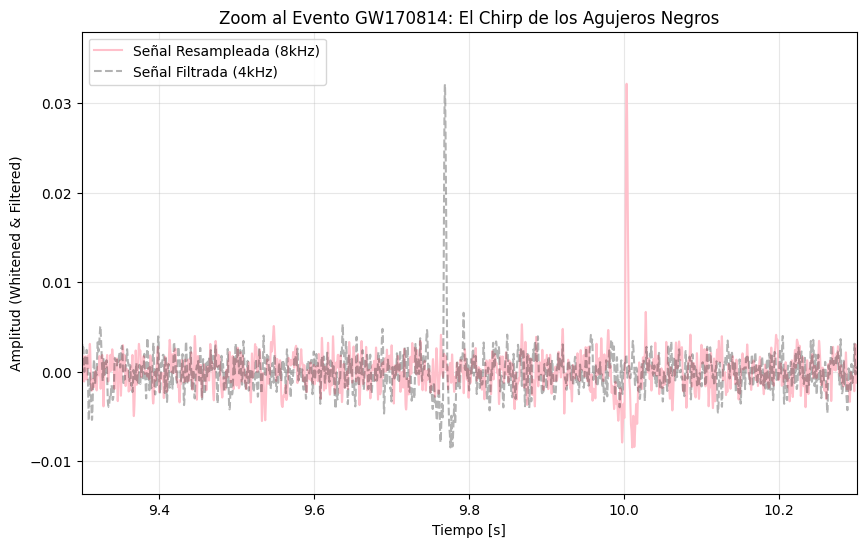
\includegraphics[width=0.45\textwidth]{amplitud.png}
    \caption{Señal procesada donde se observa el pico de amplitud y el efecto del resampleo a 8000 Hz.}
    \label{fig:amplitud}
\end{figure}
    
    \item \textbf{Análisis de Resultados:} Finalmente, se generó un espectrograma ajustando los rangos de intensidad para identificar visualmente la rampa de frecuencia del \textit{chirp}. Finalmente, se realizó la exportación de la señal procesada a formato de audio (WAV) para permitir una validación auditiva del fenómeno, permitiendo identificar el incremento de tono característico del evento astronómico..
\end{enumerate}

\section{Resultados}
Tras aplicar el flujo de procesamiento, se obtuvieron los siguientes hallazgos:
\begin{itemize}
\item \textbf{Densidad Espectral de Potencia:} La comparación inicial reveló que el uso de una ventana rectangular generaba picos de interferencia y fugas espectrales (efecto peine). La implementación de la ventana de \textit{Hann} eliminó satisfactoriamente estas anomalías, permitiendo una base limpia para el análisis de la señal.
\item \textbf{Morfología de la Onda:} En la gráfica de amplitud, se identificó un pico de energía prominente. Se observó un desplazamiento técnico del evento hacia $t \approx 10.0$ s en la señal resampleada en comparación con la señal original ($t \approx 9.77$ s). Este fenómeno se atribuye al retardo de grupo introducido por los filtros digitales utilizados durante el resampleo a $8000$ Hz.
\item \textbf{Análisis Tiempo-Frecuencia:} El espectrograma final permitió visualizar la firma del \textit{chirp} como una rampa ascendente de frecuencia. La intensidad de la señal en el intervalo de $9.8$ s a $10.0$ s sobresale notablemente sobre el ruido de fondo blanqueado, lo cual confirma la detección de la colisión de agujeros negros. Tambien la validación auditiva mediante el archivo generado a 8000 Hz permitió confirmar la presencia del \textit{chirp}. Se percibió un aumento en la frecuencia de la señal en el intervalo final, lo cual coincide con la rampa ascendente observada en el espectrograma y con la teoría de la coalescencia de agujeros negros.
\end{itemize}"
\begin{figure}[htbp]
    \centering
    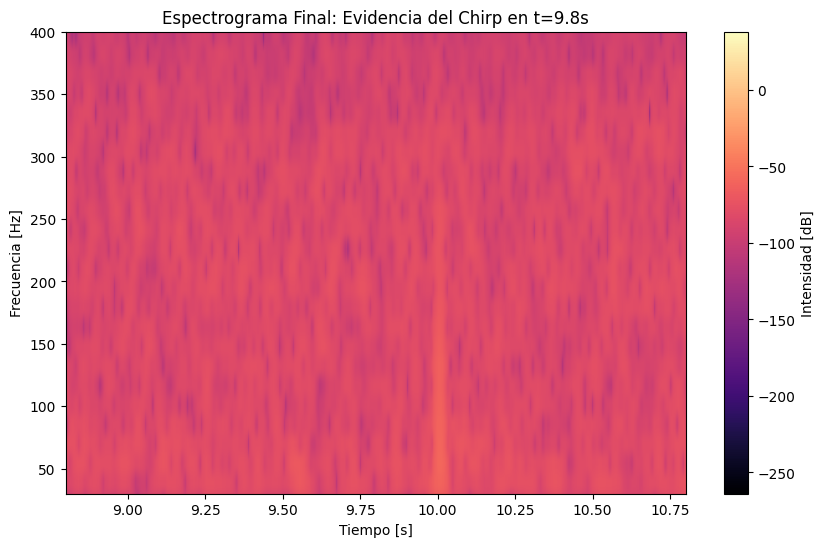
\includegraphics[width=0.45\textwidth]{espectrograma.png}
    \caption{Espectrograma final confirmando la detección del chirp del evento GW170814.}
    \label{fig:espectrograma}
\end{figure}

\section{Conclusiones}
El procesamiento digital realizado permitió aislar con éxito la señal del evento GW170814 del ruido instrumental, validando las capacidades de los detectores terrestres. Se concluye que el uso de la ventana de \textit{Hann} es un paso fundamental para obtener un análisis espectral libre de fugas y artefactos visuales \cite{oppenheim}. El flujo de trabajo aplicado facilitó la identificación del \textit{chirp} mediante una validación multimodal: visualmente a través del espectrograma y auditivamente mediante el archivo generado a 8 kHz, el cual permitió percibir con claridad el incremento de frecuencia característico de la coalescencia de agujeros negros. Finalmente, se observó que este procesamiento especializado introduce un retardo de grupo de carácter técnico que debe ser estrictamente considerado en análisis de sincronización temporal para la localización precisa de fuentes astrofísicas en el espacio profundo.




\begin{thebibliography}{1}

\bibitem{ligo2016}
B. P. Abbott et al., "Observation of Gravitational Waves from a Binary Black Hole Merger," \textit{Phys. Rev. Lett.}, vol. 116, no. 6, 2016.

\bibitem{gw170814}
B. P. Abbott et al., "GW170814: A Three-Detector Observation of Gravitational Waves from a Binary Black Hole Coalescence," \textit{Phys. Rev. Lett.}, vol. 119, no. 14, 2017.

\bibitem{oppenheim}
A. V. Oppenheim and R. W. Schafer, \textit{Discrete-Time Signal Processing}. 3rd ed. Prentice Hall, 2010.

\bibitem{gwosc}
"GW170814 Dataset," Gravitational Wave Open Science Center (GWOSC), [En línea]. Disponible en: https://gwosc.org/eventapi/html/GWTC-1-confident/GW170814/v3/.

\end{thebibliography}


\newpage





\vfill

\end{document}


